%==================================================================================================
\section{Exemplos de Verificação} \label{ExemplosMT}
%==================================================================================================

\textcolor{red}{REVISAR}

Para verificação das formulações implementadas, realizaram-se algumas simulações de problemas bidimensionais bastante conhecidos. Utilizando-se o problema de escoamento em uma cavidade, proposto por \citeonline{ghia1982high}, foi possível observar-se os impactos na solução com o uso de diferentes elementos, seguido de uma análise da convergência para tais elementos, e, por fim, uma verificação dos efeitos da inclusão de modelos de turbulência frente a uma simulação direta. Para a verificação prévia das implementações tridimensionais, adotando-se a geometria de uma cavidade tridimensional, simulou-se o problema \textit{Taylor-Green Vortex} (TGV) \cite{shapiro1993use}. Por fim, simulou-se o escoamento sobre um cilindro proposto por \citeonline{tezduyar1992incompressible,codina2006numerical,najafi2012meshless,fernandes2020tecnica}, analisando-se o comportamento transiente dos coeficientes de arrasto e de sustentação para diferentes modelos e aproximações. Os resultados obtidos para cada uma das simulações são apresentados nos Apêndices \ref{Ap:Cavity} ao \ref{Ap:cylinder}.

%==================================================================================================
\subsection{Cavidade bidimensional}
%==================================================================================================

Um problema comumente utilizado na literatura como \textit{benchmark}, trata-se de uma cavidade quadrada ($\Omega=[-1,1]^2$) com paredes aderentes, onde o fluido encontra-se confinado e sujeito a uma velocidade prescrita $\BB{u}_\infty$ ocasionada devido ao deslizamento de uma parede na face superior da cavidade. Assim são observados os efeitos provocados no escoamento devido à diferentes números de Reynolds, o qual é calculado por meio da equação \eqref{eq:Reynolds}:

\begin{equation}
    \Rey=\frac{\rho L\norm{\BB{u}_\infty}}{\mu}\text{,}
    \label{eq:Reynolds}
\end{equation}

\noindent em que $L$ é o comprimento característico, que no caso analisado é igual ao lado da cavidade. Dessa forma considera-se uma velocidade constante para todas as análises de $\BB{u}_\infty=(1,0)\trans$, sendo os diferentes números de Reynolds obtidos pela variação da viscosidade do fluido. A Figura \ref{fig:cavity} apresenta esquematicamente o problema simulado.

\begin{figure}[h!]
    \centering
    \caption{Cavidade bidimensional - Desenho esquemático}
    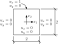
\includegraphics[width=.4\linewidth]{Figuras/Cavity/cavidade.pdf}
    \\Fonte: Autoria Própria (\the\year).
    \label{fig:cavity}
\end{figure}

Pelo fato de o problema possuir apenas fronteiras de Dirichlet, o condicionamento da solução do campo de pressões é garantido pela aplicação de uma condição de pressão nula no centro da aresta inferior da cavidade, conforme visto na figura acima. Também se observa que existe uma descontinuidade nas condições de contorno no encontro entre as paredes da cavidade e seu topo, podendo ser consideradas velocidades nulas ou igual à velocidade do topo. No problema em questão considerou-se que a velocidade nesse ponto é igual à $\BB{u}_\infty$.

A simulação foi conduzida com uma malha estruturada com orientação à esquerda pra elementos triangulares de aproximação linear e quadrática, em simulação DNS (estabilizada pelos termos PSPG, SUPG e LSIC) e com aplicação do modelo LES. A malha utilizada para a simulação de elementos lineares possui 12800 elementos enquanto para a simulação de elementos quadráticos possui 3200 elementos. Assim ambas as simulações possuirão um total de 6561 nós, o que resulta em 19683 graus de liberdade.

O fluido possui massa específica $\rho=1$ para todas as análises e viscosidade dinâmica variando de forma a se obter diferentes números de Reynolds. Assim os valores da viscosidade serão de $\mu=0,02$, $\mu=5\times10^{-3}$, $\mu=2\times10^{-3}$, $\mu=4\times10^{-4}$, $\mu=2,6667\times10^{-4}$ e $\mu=2\times10^{-4}$, resultando em $\Rey=100$, $\Rey=400$, $\Rey=1000$, $\Rey=5000$, $\Rey=7500$ e $\Rey=10000$, respectivamente. O campo de velocidades inicial em todos os casos foi de $\BB{u}=\BB{0}$, o passo de tempo foi de $\Delta t=0,1$ e a simulação foi mantida até que a estacionariedade do fluxo fosse alcançada, sendo o esquema de integração temporal obtido a partir de $\rho_\infty=0,0$. O valor da constante de Smagorinsky foi de $C_S=0,10$.

Os resultados obtidos foram comparados com aqueles apresentados por \citeonline{ghia1982high}. A Figura \ref{fig:cavity-results} apresenta os valores do campo de velocidades sobre as linhas médias da cavidade ($x_1=0$ e $x_2=0$).

\begin{figure}[h!]
    \centering
    \caption{Cavidade bidimensional - Valores do campo de velocidades sobre as linhas médias.}
    \begin{subfigure}{0.4\textwidth}
        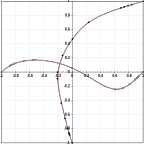
\includegraphics[width=\linewidth]{Figuras/Cavity/Re100.pdf}
        \caption{$\Rey=100$}
    \end{subfigure}
    \begin{subfigure}{0.4\textwidth}
        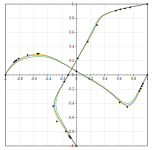
\includegraphics[width=\linewidth]{Figuras/Cavity/Re400.pdf}
        \caption{$\Rey=400$}
    \end{subfigure}
    \begin{subfigure}{0.4\textwidth}
        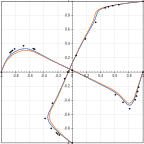
\includegraphics[width=\linewidth]{Figuras/Cavity/Re1000.pdf}
        \caption{$\Rey=1000$}
    \end{subfigure}
    \begin{subfigure}{0.4\textwidth}
        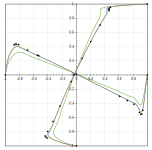
\includegraphics[width=\linewidth]{Figuras/Cavity/Re5000.pdf}
        \caption{$\Rey=5000$}
    \end{subfigure}
    \begin{subfigure}{0.4\textwidth}
        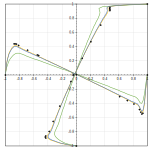
\includegraphics[width=\linewidth]{Figuras/Cavity/Re7500.pdf}
        \caption{$\Rey=7500$}
    \end{subfigure}
    \begin{subfigure}{0.4\textwidth}
        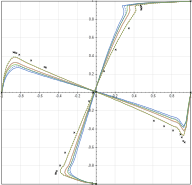
\includegraphics[width=\linewidth]{Figuras/Cavity/Re10000.pdf}
        \caption{$\Rey=10000$}
    \end{subfigure}
    \begin{subfigure}{\textwidth}
        \centering
        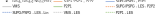
\includegraphics[width=.7\linewidth]{Figuras/Cavity/legenda.pdf}
    \end{subfigure}
    \\Fonte: Autoria Própria (\the\year).
    \label{fig:cavity-results}
\end{figure}

A Figura \ref{fig:cavity-results2} apresenta o campo de velocidades na cavidade após o escoamento atingir seu estado estacionário segundo a simulação LES utilizando elementos quadráticos.

\begin{figure}[h!]
    \centering
    \caption{Cavidade bidimensional - Campo de velocidades em regime estacionário.}
    \begin{subfigure}{0.32\textwidth}
        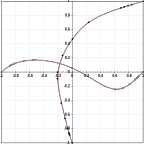
\includegraphics[width=\linewidth]{Figuras/Cavity/Re100.png}
        \caption{$\Rey=100$}
    \end{subfigure}
    \begin{subfigure}{0.32\textwidth}
        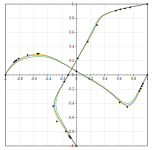
\includegraphics[width=\linewidth]{Figuras/Cavity/Re400.png}
        \caption{$\Rey=400$}
    \end{subfigure}
    \begin{subfigure}{0.32\textwidth}
        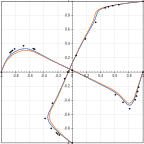
\includegraphics[width=\linewidth]{Figuras/Cavity/Re1000.png}
        \caption{$\Rey=1000$}
    \end{subfigure}
    \begin{subfigure}{0.32\textwidth}
        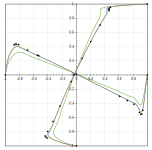
\includegraphics[width=\linewidth]{Figuras/Cavity/Re5000.png}
        \caption{$\Rey=5000$}
    \end{subfigure}
    \begin{subfigure}{0.32\textwidth}
        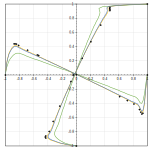
\includegraphics[width=\linewidth]{Figuras/Cavity/Re7500.png}
        \caption{$\Rey=7500$}
    \end{subfigure}
    \begin{subfigure}{0.32\textwidth}
        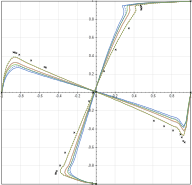
\includegraphics[width=\linewidth]{Figuras/Cavity/Re10000.png}
        \caption{$\Rey=10000$}
    \end{subfigure}
    \begin{subfigure}{0.4\textwidth}
        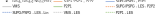
\includegraphics[width=\linewidth]{Figuras/Cavity/legenda.png}
    \end{subfigure}
    \\Fonte: Autoria Própria (\the\year).
    \label{fig:cavity-results2}
\end{figure}

Pelo fato da malha ser grosseira, percebe-se que os resultados divergem ligeiramente do esperado em relação à referência, principalmente para números de Reynolds elevados. No entanto, para esse nível de refinamento é possível observar que os elementos lineares, apesar de possuírem mesmo número de graus de liberdade, apresentaram resultados consideravelmente mais discrepantes que os elementos quadráticos. Isso se deve ao fato de que os elementos lineares não possuem a capacidade de representar adequadamente o campo de velocidades, principalmente nas regiões de maior gradiente, como é o caso das paredes da cavidade. Já, para ambos os elementos, verifica-se que a aplicação do modelo LES sobre o escoamento melhorou a representação do campo de velocidades, principalmente para números de Reynolds elevados, onde o escoamento apresenta maior turbulência. Isso deve-se ao fato do modelo ser capaz de capturar os efeitos turbulentos em escalas menores que os elementos da malha, o que não ocorre na simulação DNS.

Já com relação ao tempo de processamento, observou-se um tempo médio de 0,2285 segundos por iteração para a simulação de elementos lineares em DNS, enquanto para a simulação de elementos quadráticos o tempo médio foi de 0,2032 segundos por iteração, o que resulta em um tempo 12,466\% maior para a simulação de elementos lineares, o que mostra que mesmo possuindo um tempo de processamento maior, seus resultados são menos precisos que o elemento quadrático. Todavia, para a simulação LES, o tempo médio de processamento foi de 0,2134 segundos por iteração em elementos quadráticos, o que resulta em um tempo 5,028\% maior que a simulação DNS de elementos quadráticos, o que mostra que o modelo LES não possui um impacto significativo no tempo de processamento.

\begin{comment}
%==================================================================================================
\subsection{\textit{Taylor-Green Vortex} tridimensional}
%==================================================================================================

Para verificação dos modelos implementados em simulações tridimensionais é possível simular o problema de \textit{Taylor-Green Vortex} (TGV), o qual possui solução analítica, dada por \cite{shapiro1993use}:

\begin{subequations}
    \begin{equation}
        \begin{split}
            &\BB{u}_a(\BB{x},t)=\\
            &-\frac{Ae^{-\nu\lambda^2t}}{k^2+l^2}\begin{bmatrix}
                \lambda l\cos{(kx_1)}\sin{(lx_2)}\sin{(mx_3)}+mk\sin{(kx_1)}\cos{(lx_2)}\cos{(mx_3)} \\
                \lambda k\sin{(kx_1)}\cos{(lx_2)}\sin{(mx_3)}-ml\cos{(kx_1)}\sin{(lx_2)}\cos{(mx_3)} \\
                -(k^2+l^2)\cos{(kx_1)}\cos{(lx_2)}\sin{(mx_3)}
            \end{bmatrix}\text{,}
        \end{split}
    \end{equation}
    \begin{equation}
        p_a=p_s-\rho\frac{u_1^2+u_2+u_3^2}{2}\text{.}
    \end{equation}
\end{subequations}

\noindent em que $k$, $l$ e $m$ são constantes arbitrárias, $\lambda^2=k^2+l^2+m^2$, $A$ é a amplitude da componente $u_3$ e $p_s$ é a pressão do ponto de estagnação.

Para o problema numérico foi considerado um cubo ($\Omega=[-1,1]^3$) simulado nos modelos VMS de aproximação linear e quadrática e o LES utilizando elementos Taylor-Hood P2P1. A malha utilizada na discretização conta com 5802 elementos finitos (conforme ilustrado na Figura \ref{fig:TGV-mesh}), sendo 5580 graus de liberdade para VMS linear, 37600 pra VMS quadrático e 29595 para LES.

\begin{figure}[h!]
    \centering
    \caption{Malha utilizada para a simulação de TGV.}
    \includegraphics[width=0.4\linewidth]{Figuras/taylor-green/mesh.png}
    \\Fonte: Autoria Própria (\the\year).
    \label{fig:TGV-mesh}
\end{figure}

Como condição inicial impôs-se acelerações, velocidade e pressões iguais à solução analítica com $t=0$ e como condições de contorno aplicou-se velocidades iguais à analítica em toda a fronteira e $p=0$ no centro do domínio. Os valores dos parâmetros foram $k=l=m=\pi$ e $A=\nu=\rho=1$, sendo o período analisado de $t\in[0,0.2]$ com um passo de tempo de $\Delta t=0.001$.

Sendo assim, a Figura \ref{fig:TGV-results} apresenta os valores do campo de velocidades nas linhas $x_2=x_3=0$ ($l1$), $x_1=x_3=0$ ($l2$) e $x_1=x_2=0$ ($l3$) para os instantes $t=0$, $t=0.05$ e $t=0.2$ para todos os modelos considerados.

\begin{figure}[h!]
    \centering
    \caption{Velocidades obtidas na simulação de TGV em:}
    \begin{subfigure}{0.42\textwidth}
        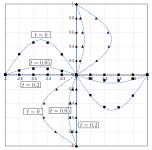
\includegraphics[width=\linewidth]{Figuras/taylor-green/VMS-Lin.pdf}
        \caption{$l1$ e $l2$ para VMS linear.}
    \end{subfigure}
    \begin{subfigure}{0.42\textwidth}
        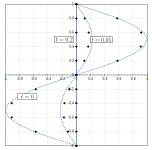
\includegraphics[width=\linewidth]{Figuras/taylor-green/VMS-Lin-uz.pdf}
        \caption{$l3$ para VMS linear.}
    \end{subfigure}
    \begin{subfigure}{0.42\textwidth}
        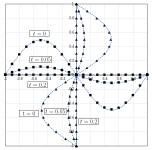
\includegraphics[width=\linewidth]{Figuras/taylor-green/VMS-Qua.pdf}
        \caption{$l1$ e $l2$ para VMS quadrático.}
    \end{subfigure}
    \begin{subfigure}{0.42\textwidth}
        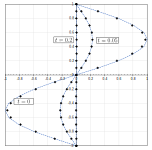
\includegraphics[width=\linewidth]{Figuras/taylor-green/VMS-Qua-uz.pdf}
        \caption{$l3$ para VMS quadrático.}
    \end{subfigure}
    \begin{subfigure}{0.42\textwidth}
        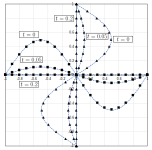
\includegraphics[width=\linewidth]{Figuras/taylor-green/LES.pdf}
        \caption{$l1$ e $l2$ para LES.}
    \end{subfigure}
    \begin{subfigure}{0.42\textwidth}
        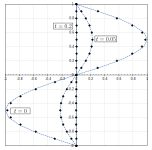
\includegraphics[width=\linewidth]{Figuras/taylor-green/LES-uz.pdf}
        \caption{$l3$ para LES.}
    \end{subfigure}
    \begin{subfigure}{0.42\textwidth}
        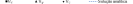
\includegraphics[width=\linewidth]{Figuras/taylor-green/legenda.pdf}
    \end{subfigure}
    \\Fonte: Autoria Própria (\the\year).
    \label{fig:TGV-results}
\end{figure}

Para comparação com a solução analítica, tomou-se a medida do erro em $L^2$, expresso por \cite{dumon2011proper}:

\begin{equation}
    \norm{\BB{e}}=\norm{\BB{u}-\BB{u}_a}_{L^\infty(L^2(\Omega))}=\max_{0<t\leq T}{\left[\int_\Omega{\norm{\BB{u}-\BB{u}_a}^2d\Omega}\right]}\text{,}
\end{equation}

\noindent o qual é representado ao longo do tempo de acordo com a Figura \ref{fig:TGV-L2}:

\begin{figure}[h!]
    \centering
    \caption{Medidas de $L^2$ ao longo do tempo.}
    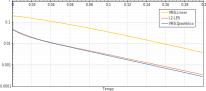
\includegraphics[width=\linewidth]{Figuras/taylor-green/L2.pdf}
    \\Fonte: Autoria Própria (\the\year).
    \label{fig:TGV-L2}
\end{figure}

Assim, observa-se que para o problema estudado, tanto as simulações VMS de aproximação quadrática quanto LES com elemento P2P1 apresentaram boa concordância com o resultado analítico, sendo que ambos apresentaram erros muito próximos entre si, enquanto o VMS de aproximação linear já apresentou um erro maior. Analisando o instante de tempo $t=0.1$ obteve-se um erro $L^2$ de $3,55\times 10^{-2}$, $2,77\times 10^{-3}$ e $3,07\times 10^{-3}$ para as simulações VMS linear, quadrático e LES, respectivamente. Ao verificar a ordem da medida do erro, observa-se que estes valores se encontram próximos ao obtido por \citeonline{zapata2023parallel}. Realizando uma regressão exponencial do tipo \[\norm{\BB{e}}=a\cdot10^{mt}\] para $t\geq 0,1$, encontra-se $m=-9,80$, $m=-10,01$ e $m=-9,60$ para os respectivos modelos.
\end{comment}

\newpage
%==================================================================================================
\subsection{Escoamento em degrau invertido}
%==================================================================================================

O problema de escoamento em degrau invertido é um problema clássico de escoamento em dutos, sendo bastante utilizado como \textit{benchmark} \cite{armaly1983experimental,chiang1999numerical}. O problema consiste em um escoamento advindo de um duto, cuja seção sofre um alargamento abrupto, conforme ilustrado na Figura \ref{fig:step}. Tal problema tem sua origem nos estudos experimentais de \citeonline{armaly1983experimental} e posteriormente estudado numericamente em problemas tridimensionais por \citeonline{chiang1999numerical}.

\begin{figure}[h!]
    \centering
    \caption{Escoamento em degrau invertido - Desenho esquemático.}
    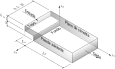
\includegraphics[width=.7\linewidth]{Figuras/backwardFacingStep/backwardFacingStep.pdf}
    \\Fonte: Autoria Própria (\the\year).
    \label{fig:step}
\end{figure}

Em seu estudo numérico, \citeonline{chiang1999numerical} considerou um duto de largura constante $B$, uma altura de seção transversal a montante de $h$ e comprimento $L_u$, e altura a jusante de $H=h+S$ com comprimento $L_d$. Nas laterais do duto considerou-se paredes aderentes, ou seja, $\BB{u}=\BB{0}$, assim como nas faces do fundo e do topo do duto. Na face de entrada do duto considerou-se uma velocidade prescrita $\BB{u}_\infty=(u_1(x_2,x_3),0,0)\trans$, tal que:

\begin{subequations}
    \begin{equation}
        u_1(x_2,x_3)=\frac{48}{\alpha\pi^3}\beta(x_1,x_2)\text{,}
    \end{equation}
    \begin{equation}
        \alpha=1-\frac{192B}{\pi^5}\sum_{i=1,3,5,\hdots}^{\infty}\frac{\tanh{(\xi_i)}}{i^5}\text{,}
    \end{equation}
    \begin{equation}
        \beta(x_1,x_2)=\sum_{i=1,3,5,\hdots}^{\infty}(-1)^{(i-1)/2}\bigpar{1-\frac{\cosh{[(2x_2-1)\xi_i]}}{\cosh{(\xi_i)}}}\frac{\cos{(2x_3\xi_i)}}{i^3}\text{ e}
    \end{equation}
    \begin{equation}
        \xi_i=\frac{\pi i}{2B}\text{.}
    \end{equation}
\end{subequations}

Devido à simetria do problema, considerou-se somente metade da largura do duto, impondo-se uma condição de simetria ($u_3=0$) no plano $x_3=0$, o qual é utilizado para observar os resultados do problema.

Para a simulação numérica, considerou-se um duto com largura $B=35h$, altura $h=1,0$, altura do degrau $S=0,9423$ e comprimento $L_u=0,0$ e $L_d=55,0$. A malha utilizada na discretização do domínio foi construída a partir de elementos tetraédicos de aproximação quadrática de tamanho 0,5 na região de entrada do duto e 0,6 na região de saída. Assim obtém-se uma malha com 57173 elementos finitos e 95334 nós, resultando em 381336 graus de liberdade (conforme ilustrado na Figura \ref{fig:step-mesh}). A simulação foi estabilizada a partir da estabilização SUPG/PSPG.

\textcolor{red}{FIGURA}

O número de Reynolds do problema analisado é obtido a partir da equação \eqref{eq:ReyBFS}:

\begin{equation}
    \Rey=\frac{\rho u_\mathrm{médio}(2h)}{\mu}\text{,}
    \label{eq:ReyBFS}
\end{equation}

\noindent sendo $u_\mathrm{médio}=1,0$ a velocidade média na região de entrada do duto. Assim, sendo $\rho=1,0$, considera-se os valores de viscosidade dinâmica $\mu=0,02$, $5,1414\times10^{-3}$ e $2,0\times10^{-3}$, o que resulta em $\Rey=100$, $389$ e $1000$, respectivamente. O passo de tempo foi de $\Delta t=0,1$ e a simulação foi mantida até que a estacionariedade do fluxo fosse alcançada, sendo o esquema de integração temporal obtido a partir de $\rho_\infty=0,0$.

Além disso, uma simulação bidimensional foi conduzida para o $\Rey=1000$, uma vez que \citeonline{chiang1999numerical} observaram uma discrepância entre os valores de simulações bidimensionais e tridimensionais para esse número de Reynolds. Como mencionado pelos autores, essa diferença se dá pela influência da parede aderente nos resultados, o que não é capturada pela simulação bidimensional.

A malha utilizada para a simulação bidimensional foi construída a partir de elementos triangulares de aproximação quadrática de tamanho 0,5 na região de entrada do duto e 0,6 na região de saída. Assim obtém-se uma malha com 836 elementos finitos e 1883 nós, resultando em 5649 graus de liberdade.

A Figura \ref{fig:BFSvel} apresenta os perfis de velocidade para diferentes distâncias ao longo da linha de fluxo para as três simulações conduzidas.

\begin{figure}[h!]
    \centering
    \caption{Escoamento em degrau invertido - Perfis de velocidade.}
    \begin{subfigure}{0.75\textwidth}
        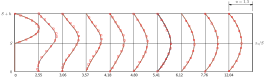
\includegraphics[width=\linewidth]{Figuras/backwardFacingStep/Re100.pdf}
        \caption{$\Rey=100$}
    \end{subfigure}
    \begin{subfigure}{0.75\textwidth}
        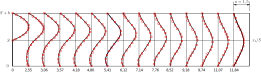
\includegraphics[width=\linewidth]{Figuras/backwardFacingStep/Re389.pdf}
        \caption{$\Rey=389$}
    \end{subfigure}
    \begin{subfigure}{0.75\textwidth}
        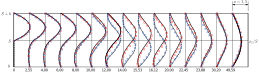
\includegraphics[width=\linewidth]{Figuras/backwardFacingStep/Re1000.pdf}
        \caption{$\Rey=1000$}
    \end{subfigure}
    \begin{subfigure}{0.3\textwidth}
        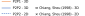
\includegraphics[width=\linewidth]{Figuras/backwardFacingStep/legenda.pdf}
    \end{subfigure}
    \\Fonte: Autoria Própria (\the\year).
    \label{fig:BFSvel}
\end{figure}

Outra simulação realizada trata-se do problema bidimensional com $S=1$ e $\Rey=800$, onde os autores observaram os perfis de velocidade para as distâncias $x_1=14$ e $x_1=30$, além da distribuição de pressões ao longo do fundo e do topo do canal. Como a pressão de estagnação do problema simulado é nula na face de saída do duto, foi apenas adicionada uma pressão constante nos resultados de referência para fins de comparação, de forma que as pressões sejam equivalentes nesse ponto especificado. As Figuras \ref{fig:BFS800-vel} e \ref{fig:BFS800-pre} apresentam os resultados obtidos para a simulação bidimensional.

\begin{figure}[h!]
    \centering
    \caption{Escoamento em degrau invertido - Perfis de velocidade para $\Rey=800$.}
    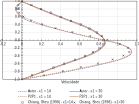
\includegraphics[width=.6\linewidth]{Figuras/backwardFacingStep/resultado2D-2.pdf}
    \\Fonte: Autoria Própria (\the\year).
    \label{fig:BFS800-vel}
\end{figure}

\begin{figure}[h!]
    \centering
    \caption{Escoamento em degrau invertido - Distribuição de pressões para $\Rey=800$.}
    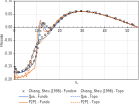
\includegraphics[width=.6\linewidth]{Figuras/backwardFacingStep/resultado2D-1.pdf}
    \\Fonte: Autoria Própria (\the\year).
    \label{fig:BFS800-pre}
\end{figure}

Assim, percebe-se boa concordância com os resultados obtidos pela referência, tanto para os perfis de velocidade em $\Rey=100$, $389$, $800$ e $1000$, quanto para a distribuição de pressões em $\Rey=800$.